\documentclass[table]{beamer}
\usepackage{xcolor}
\usepackage{tikz}
\usepackage{pgfplots}
\usepackage{graphicx}
\usepackage{tabu}
\usepackage{booktabs}
\usepackage{fontawesome}
\usepackage{amsmath}

\usetikzlibrary{positioning}
\usetikzlibrary{calc}
%\usetikzlibrary{arrows}

\usefonttheme{professionalfonts}
\usetheme{Boadilla}
\setbeamertemplate{navigation symbols}{}%remove navigation symbols
\hypersetup{pdfstartview={Fit}} % fits the presentation to the window when first displayed
\graphicspath{{./figures/}{../ch2/figures/}{../ch3/figures/}{../ch4/figures/}{../ch5/figures/}}
\definecolor{gold}{rgb}{1,.776,.153}
\definecolor{maroon}{rgb}{.549,.114,.251}

%Info
\title[Mutations in Non-model Organisms]{Methods for Detecting Mutations in Non-model Organisms}
\titlegraphic{
	\includegraphics[width=.3\linewidth]{emel_1.jpg}
	}
\date{11/6/20}
\author{Adam Orr}


\begin{document}
\frame{\titlepage}

\begin{frame}{Why Care About Mutations and Genotyping?}
\begin{columns}

\column{.5\linewidth}
\textbf{Human Health}
\begin{itemize}
\item Cancer
\item Personalized Medicine
\end{itemize}

\vfill

\textbf{Agriculture}
\begin{itemize}
\item Looking for interesting phenotypes in clonally reproducing species
\item Breeding programs
\end{itemize}

\textbf{Evolution}
\begin{itemize}
\item Mutations are the ultimate source of variation
\item Mutation rate diversity and evolution
\end{itemize}

\column{.5\linewidth}
\includegraphics[width=\linewidth]{nectarine.jpg}

\end{columns}
\footnotetext{\tiny{\url{https://commons.wikimedia.org/wiki/File:White_nectarine_and_cross_section02_edit.jpg}}}
\end{frame}


\begin{frame}{Mutations can be difficult to detect}

\begin{block}{Mutations are very rare, but sequencing errors are very common.}
\textbf{Sequencing error} alone is \textbf{$\sim10^{-3}$} while mutation rate after error-checking is \textbf{$\sim10^{-9}$}
\end{block}

% TODO: i think here i should show an example alignment. instead of this.
\begin{itemize}
\item Errors accumulate during PCR prior to sequencing - then propagate.
\item \textit{Taq} $\sim10^{-4}$
\item Technical error from sequencer
\end{itemize}

\includegraphics[trim={1cm 4cm 0 0},clip,width=\linewidth]{pcr_errors.png}

\footnotetext{\tiny{Potapov V, Ong JL (2017) Examining Sources of Error in PCR by Single-Molecule Sequencing}}
\end{frame}

\begin{frame}{Working with Non-model Organisms can be difficult}

\begin{itemize}
	\item No reference genome
	\item Many methods assume a reliable reference and other supporting information
	\item Assembling your own is possible but unsatisfying; costly and time-consuming to do well
	\item 50,000 species in NCBI genome database of 600,000 in taxonomy database; few are reference quality
	\item We need robust reference-free methods!
\end{itemize}

\end{frame}


\begin{frame}{How does plant growth affect somatic mutation rate?}

We want to understand mutation patterns within a non-model organism.

\begin{columns}
	\column{.5\linewidth}
		\includegraphics[trim={12cm 2cm 0 22cm},clip,width=.8\linewidth]{stemcells.jpg}
	\column{.5\linewidth}
		\begin{itemize}
			\item The genetic structure of the plant \textit{should} mirror its physical structure.
		\end{itemize}
\end{columns}
\footnotetext{Heidstra \& Sabatini (2014) Plant and animal stem cells: similar yet different. doi:10.1038/nrm3790}
\end{frame}

\begin{frame}{A Genetic Mosaic}
	\begin{center}
	\includegraphics[width=.5\linewidth]{emel_1.jpg}
	\end{center}
	\begin{itemize}
		\item Mosaic: differential oil production gives protection from beetles
		\item Does the pattern of mutation match the physical structure?
		\item Can we detect enough mutations to measure the mutation rate?
	\end{itemize}
	\footnotetext{Orr et al. (2020) A phylogenomic approach reveals a low somatic mutation rate in a long-lived plant. doi:10.1098/rspb.2019.2364}
\end{frame}

\begin{frame}{Current reference-free methods are insufficient}
\begin{columns}
	\column{.5\linewidth}
		\includegraphics[width=\linewidth]{01-first-11-scaffolds.pdf}
	\column{.5\linewidth}
	\begin{itemize}
		\item Sequence 8 samples in triplicate
		\item $\sim$10X coverage for each replicate
		\item DiscoSNP++ uses small differences in similar sequencing reads to find potential mutations
		\item Coverage may not be sufficient for this method
		\item The repetitive nature of the genome may make it difficult to differentiate repeated DNA from mutations
	\end{itemize}
\end{columns}
\end{frame}

\begin{frame}{Approximating a Genome}
Use \textit{E. grandis} genome as a starting place, then generate a new reference and map to that reference.
\begin{center}
	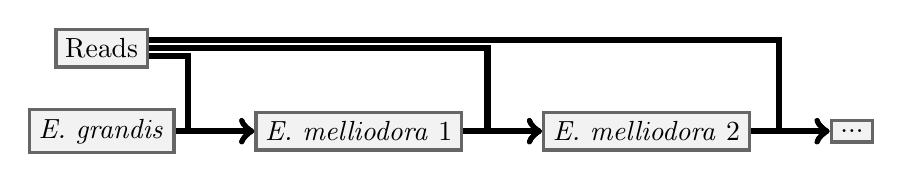
\begin{tikzpicture}[cnode/.style={rectangle,draw=black!60,fill=black!5,very thick}, node distance = 1 cm]
		\node[cnode] (reads){Reads};
		\node[cnode] (eg)[below = .5cm of reads]{\textit{E. grandis}};
		\node[cnode] (em1)[right = of eg]{\textit{E. melliodora} 1};
		\node[cnode] (em2)[right = of em1]{\textit{E. melliodora} 2};
		\node[cnode] (etc)[right = of em2] {...};
		\draw[line width=.8mm,->] ($(reads.east)-(0cm,.1cm)$) -- ($(reads.east)+(.5cm,-.1cm)$) |- (em1.west);
		\draw[line width=.8mm,->] (reads.east) -- ($(reads.east)+(4.3cm,0cm)$) |- (em2.west);
		\draw[line width=.8mm,->] ($(reads.east)+(0cm,.1cm)$) -- ($(reads.east)+(8cm,.1cm)$) |- (etc.west);
		\draw[line width=.8mm,->] (eg) -- (em1);
		\draw[line width=.8mm,->] (em1) -- (em2);
		\draw[line width=.8mm,->] (em2) -- (etc);
	\end{tikzpicture}
\end{center}
\end{frame}

\begin{frame}{Analysis Pipeline}
\begin{columns}
\column{.5\linewidth}
\begin{itemize}
\item Sequence 8 samples in triplicate
\item Align sequence to the edited \textit{Eucalyptus grandis} genome
\item Use replicates to remove false positives
\end{itemize}
\column{.5\linewidth}
\begin{center}
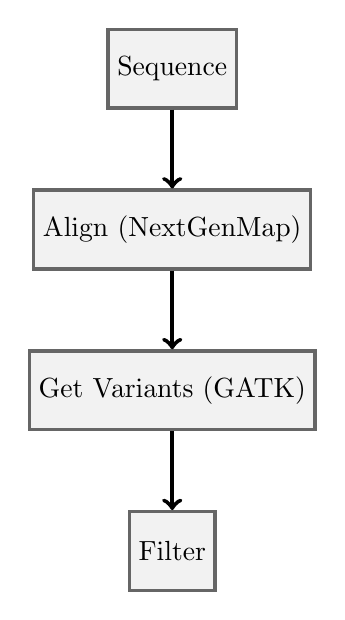
\begin{tikzpicture}[sqnode/.style={rectangle, draw=black!60, fill=black!5,very thick,minimum size=1cm}]
	\node[sqnode] (sequencing) {Sequence};
	\node[sqnode] (alignment) [below = of sequencing] {Align (NextGenMap)};
	\node[sqnode] (varcall) [below = of alignment] {Get Variants (GATK)};
	\node[sqnode] (flt) [below = of varcall] {Filter};
	\draw[ultra thick,->] (sequencing.south) -- (alignment.north);
	\draw[ultra thick,->] (alignment.south) -- (varcall.north);
	\draw[ultra thick,->] (varcall.south) -- (flt.north);
\end{tikzpicture}
\end{center}
\end{columns}
\end{frame}

\begin{frame}{Pipeline Produces Tree Close to Physical Tree}
	\includegraphics[width=\linewidth]{emel_2.jpg}
	\footnotetext{Orr et al. (2020) A phylogenomic approach reveals a low somatic mutation rate in a long-lived plant. doi:10.1098/rspb.2019.2364}
\end{frame}

\begin{frame}{Using Tree Topology Gives Higher Recall Rate}
	\begin{itemize}
	\item Thus, it's reasonable to assume the physical topology when inferring mutations
	\item \textit{DeNovoGear} is a variant-calling method that uses information in the tree topology to call variants.
	\item By simulation, we introduced 14000 mutations on the tree
	\end{itemize}
	\begin{center}
	\begin{tabular}{ c | c }
	\textit{GATK} & \textit{DeNovoGear} \\
	\hline
	3859 mutations & 4193 mutations \\
	27\% & 30\%
	\end{tabular}
	\end{center}
\end{frame}

\begin{frame}{Using Random Trees to Estimate False Positive Rate}
\begin{itemize}
	\item If we assume mutations should match the tree structure, no real mutations should also match a random maximally-distant tree.
	\item Simulate 100 trees maximally distant from the true tree and ask how many the pipeline detects on average.
\end{itemize}
\begin{center}
\begin{tabular}{ c | c }
	\textit{GATK} & \textit{DeNovoGear} \\
	\hline
	55.71 of 99 mutations & .11 of 90 mutations \\
	56.3\% & .12\%
\end{tabular}
\end{center}
\end{frame}


\begin{frame}{Mutation Rates}
\begin{columns}
\column{.5\linewidth}
\begin{itemize}
\item Detected $90$ mutations.
\item $20$ mutations in genes.
\item Estimated recall of $\sim30\%$.
\item $90\times\frac{1}{.3}=300$ mutations.
\item $\sim3.3$ mutations per meter of length
\item $2.7\times10^{-9}$ mutations per base per meter
\item Somatic mutations account for $\sim55$ mutations per leaf tip.
\end{itemize}
\column{.5\linewidth}
\includegraphics[width=\linewidth]{emel_1.jpg}
\end{columns}
\end{frame}

\begin{frame}{Population Estimates}
\begin{columns}
\column{.5\linewidth}
We studied \textit{one} individual, but we can make conjectures about the population.
\begin{itemize}
\item The average height of a eucalypt is $22.5$ M
\item Mutation rate per base, per generation from somatic mutation is $6.2\times10^{-8}$
\item We estimated $\theta = 0.025$
\item Since $\theta = 4N_{e}\mu$, $N_{e} = 102,000$
\end{itemize}
\column{.5\linewidth}
\includegraphics[width=\linewidth]{emel_1.jpg}
\\
\end{columns}

\vskip 1em

\hrule

\vskip 1em

This per-generation rate is $\sim10\times$ larger than \textit{Arabidopsis}, but \textit{Eucalyptus} is $100\times$ larger.

\end{frame}



% Base Quality Scores

\begin{frame}[fragile]{How do we do better? Base Quality Scores help find errors}

Errors make variant calling difficult - but we can predict them.

\begin{itemize}
	\item FASTQ format data has a quality score
	\item Quality scores represent $P(error)$ on a phred scale.
\end{itemize}

\begin{displaymath}
	P(error) = 10^{\frac{-Q}{10}}
\end{displaymath}
\begin{displaymath}
	Q = -10\log_{10}{P(error)}
\end{displaymath}

\begin{block}{FASTQ Example}
\begin{verbatim}
@SEQ_ID
GATTTGGGGTTCAAAGCAGTATCGATCAAATAGTAAATCCATTTGTTCAACTCACAGTTT
+
!''*((((***+))%%%++)(%%%%).1***-+*''))**55CCF>>>>>>CCCCCCC65
\end{verbatim}
\end{block}

\footnotetext{\url{https://en.wikipedia.org/wiki/FASTQ_format}}

\end{frame}

\begin{frame}{Quality scores are predictions}
\begin{columns}
\column{.5\linewidth}
\begin{itemize}
\item A quality score is a \textbf{prediction} about whether a base call is correct.
\item Predictions are said to be \textbf{calibrated} if the predicted event occurs as often as predicted.
\item The weather forecast contains a \textbf{prediction} about whether it will rain.
\item If it rains on a day with a 30\% chance of rain, what does that mean?
\end{itemize}
\column{.5\linewidth}
\begin{tikzpicture}
\begin{axis}[width = .9\textwidth, xlabel={Predicted Probability}, ylabel={Measured Frequency}]
\addplot[black,samples = 50,domain=0:1]{x};
\end{axis}
\end{tikzpicture}
\end{columns}
\end{frame}

\begin{frame}{Quality scores aren't well-calibrated}
\begin{columns}
\column{.5\linewidth}
\begin{itemize}
\item If quality scores \textit{were} well-calibrated, it would be easier to identify errors
\item Base Quality Score Recalibration can be done to fix calibration issues.
\item GATK method for BQSR require a database of variable sites in your data
then assumes mismatches at nonvariable sites are errors.
\end{itemize}
\column{.5\linewidth}
\includegraphics[width=.95\linewidth]{gatk_comparison.pdf}
\end{columns}
\end{frame}


\begin{frame}{Base Quality Score Recalibration}

GATK BQSR is the standard method for BQSR. It works in 3 phases:

\begin{enumerate}
	\item Find errors with alignment
	\item Train model
	\item Recalibrate with model
\end{enumerate}

\hskip 1em


%table stuff
\newcolumntype{y}{>{\columncolor{yellow}} c}
\newcolumntype{x}{>{\columncolor{red}} c}
\newcolumntype{z}{>{\columncolor{cyan}} c}


\begin{tabular}{r c c c z c c c c c c}
Reference & A & T & G & C & T & A & A & G & C & A\\
\hline
& &T &G &T & & & & & & \\
& & &\cellcolor{red}T & T& T& & & & & \\
& & & &T & T& A& & & & \\
\end{tabular}

\hskip 1em

One site is excluded and one base is an error. $\frac{1}{6}$ bases is an error.

\end{frame}

\begin{frame}{GATK BQSR is difficult in non-model organisms}

\begin{itemize}
	\item Many mismatches between reference and sample (if there is one)
	\item No database with sites to exclude
\end{itemize}

\hskip 1em
%table stuff
\newcolumntype{y}{>{\columncolor{yellow}} c}
\newcolumntype{x}{>{\columncolor{red}} c}
\newcolumntype{z}{>{\columncolor{cyan}} c}

\begin{tabular}{r c c c x c c c c c c}
Reference & A & T & G & C & T & A & A & G & C & A\\
\hline
& &T &G &T & & & & & & \\
& & &\cellcolor{red}T & T& T& & & & & \\
& & & &T & T& A& & & & \\
\end{tabular}

\hskip 1em

One site isn't excluded; only one base is really an error. $\frac{4}{9}$ bases are estimated to be errors.

\end{frame}

%%how does miscalibration affect variant calling ? use bcftools model example

\begin{frame}{GATK BQSR uses a hierarchical linear model to determine how much to adjust each quality score}
\centering
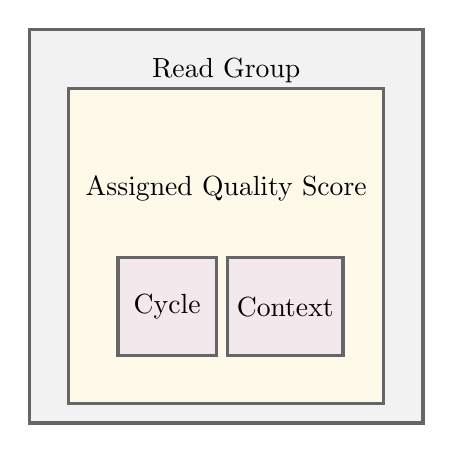
\begin{tikzpicture}[align=center, sqnode/.style={rectangle,draw=black!60,fill=black!5,very thick,minimum size=1cm}, node distance = 1 cm]
	\node[sqnode,align=center,above,minimum size=5cm](rg) at (2,0){};
	% \draw[help lines] (0,0) grid (16,16);
	\node[](rglab) at (2,4.5){Read Group};
	\node[sqnode, align=center,above,minimum size=4cm,fill=gold!10](q) at (2,.25){};
	\node[](qlab) at (2,3){Assigned Quality Score};
	\node[sqnode, minimum size = 1.25 cm,fill=maroon!10] at (1.25,1.5) {Cycle};
	\node[sqnode, minimum size = 1.25 cm,fill=maroon!10] at (2.75,1.5) {Context};
\end{tikzpicture}
\end{frame}

\begin{frame}{Example Recalibration}
\includegraphics[width = \linewidth]{recalibration_explainer.pdf}
\end{frame}



\begin{frame}{GATK BQSR uses a hierarchical linear model to determine how much to adjust each quality score}

\begin{displaymath}
Q = \bar{Q} + \Delta RG + \Delta{} Q + \Delta{} C (Cycle) + \Delta{} X (Context)
\end{displaymath}

\begin{displaymath}
\Delta{}RG = argmax_{q}\{P(\mathcal{B}(RG_{t},q) = RG_{e}) * P(\mathcal{N}(\bar{Q}) = q)\} - \bar{Q}
\end{displaymath}

\begin{displaymath}
\Delta Q = argmax_{q}\{P(\mathcal{B}(Q_{t},q) = Q_{e}) * P(\mathcal{N}(\bar{Q} + \Delta RG) = q)\} - (\bar{Q} + \Delta RG)
\end{displaymath}

\begin{multline}
\Delta Cycle = argmax_{q}\{P(\mathcal{B}(C_{t},q) = C_{e}) * P(\mathcal{N}(\bar{Q} + \Delta RG + \Delta Q) = q)\} \\ - (\bar{Q} + \Delta RG + \Delta Q)
\end{multline}

\begin{multline}
\Delta Context = argmax_{q}\{P(\mathcal{B}(X_{t},q) = X_{e}) * P(\mathcal{N}(\bar{Q} + \Delta RG + \Delta Q) = q)\} \\ - (\bar{Q} + \Delta RG + \Delta Q)
\end{multline}

\end{frame}


% \begin{frame}{BQSR resilient to simulated false positives}
% \centering
% \includegraphics[width=.65\linewidth]{fpr.pdf}

% %table stuff
% \newcolumntype{y}{>{\columncolor{yellow}} c}
% \newcolumntype{x}{>{\columncolor{red}} c}
% \newcolumntype{z}{>{\columncolor{cyan}} c}

% \begin{tabular}{r z c c z c c z c c c}
% Reference & A & T & G & C & T & A & A & G & C & A\\
% \hline
% & &T &G &T & & & & & & \\
% & & &\cellcolor{red}T & T& T& & & & & \\
% & & & &T & T& A& & & & \\
% \end{tabular}

% \end{frame}

\begin{frame}{BQSR vulnerable to simulated false negatives}
\centering
\includegraphics[width=.65\linewidth]{fnr.pdf}

%table stuff
\newcolumntype{y}{>{\columncolor{yellow}} c}
\newcolumntype{x}{>{\columncolor{red}} c}
\newcolumntype{z}{>{\columncolor{cyan}} c}

\begin{tabular}{r c c c x c c c c c c}
Reference & A & T & G & C & T & A & A & G & C & A\\
\hline
& &T &G &T & & & & & & \\
& & &\cellcolor{red}T & T& T& & & & & \\
& & & &T & T& A& & & & \\
\end{tabular}

\end{frame}

\begin{frame}{Alternative approaches get around using a database of variable sites}
\begin{itemize}
	\item SOAP2 has a consensus calling model that performs BQSR
	\item ReQON limits the number of errors there can be at a site
	\item Synthetic spike-ins
	\item GATK Recommended method: Use the best reference you can get, call a confident set of variants, and use that.
\end{itemize}
\end{frame}

\begin{frame}{Let's find errors with k-mers instead of an alignment}

\begin{itemize}
\item Error correction methods exist that use k-mers to identify errors rather than an alignment and reference.
\item Most error correctors don't update quality scores; \texttt{Lighter} optionally updates quality scores of corrections to a value but this doesn't materially affect the calibration.
\end{itemize}

%at least a few slides explaining how Lighter works
\end{frame}

\begin{frame}{Error Detection with Lighter}
\begin{enumerate}
	\item Subsample k-mers at rate $\alpha$
	\item Use subsampled k-mers to find trusted k-mers
	\item Use trusted k-mers to correct untrusted k-mers
\end{enumerate}

\newcolumntype{y}{>{\columncolor{yellow}} c}
\newcolumntype{x}{>{\columncolor{red}} c}
\newcolumntype{z}{>{\columncolor{cyan}} c}

\begin{tabular}{r c c c c c c c c c c}
Read & A & T & G & C & T & A & A & G & C & A\\
\hline
Kmer 1& A&T &G & & & & & & & \\
Kmer 2& & \cellcolor{cyan}T&\cellcolor{cyan}G &\cellcolor{cyan}C& & & & & & \\
Kmer 3& & & G&C & T& & & & & \\
\end{tabular}

\end{frame}

\begin{frame}{Subsampling}
\newcolumntype{y}{>{\columncolor{yellow}} c}
\newcolumntype{x}{>{\columncolor{red}} c}
\newcolumntype{z}{>{\columncolor{cyan}} c}

\begin{tabular}{r c c c c c c c c c c}
Read & A & T & G & C & T & A & A & G & C & A\\
\hline
Kmer 1& A&T &G & & & & & & & \\
Kmer 2& & \cellcolor{cyan}T&\cellcolor{cyan}G &\cellcolor{cyan}C& & & & & & \\
Kmer 3& & & G&C & T& & & & & \\
\end{tabular}

\vskip 1em

Keep each k-mer with probability $\alpha$. If the same sequence is sequenced $M$ times, that k-mer will appear multiple times. The probability we sample it is then $1-(1-\alpha)^M$

\vskip 1em

\begin{tabular}{r c c c c c c c c c c}
Copy 1& A & T & G &  &  &  &  &  &  & \\
Copy 2& A& T &G & & & & & & & \\
Copy 3& A& T&G & & & & & & & \\
\end{tabular}

P(not sampled) = $(1 - \alpha)^3$ so P(sampled) = $1 - (1 - \alpha)^3$

\end{frame}

\begin{frame}{Trusting K-mers}
If we \textbf{assume an error will only show up at most twice}, the probability an erroneous k-mer is sampled is $1 - (1 - \alpha)^2$

\hskip 1em

Each base pair has between 1 and k associated k-mers; we can do a binomial test to determine whether the number of sampled k-mers associated with a base pair is too high for it to be an error:
\begin{displaymath}
P(\mathcal{B}(covering, 1 - (1-\alpha)^2) = sampled) > .95
\end{displaymath}

When there are $K$ base-pairs that are trusted, we add this to a set of trusted k-mers.

\end{frame}

\begin{frame}{Finding Errors in reads}

Given the set of trusted k-mers, find the longest stretch of trusted k-mers in the read. Then, the bases that border this stretch are errors.

\newcolumntype{y}{>{\columncolor{yellow}} c}
\newcolumntype{x}{>{\columncolor{red}} c}
\newcolumntype{z}{>{\columncolor{cyan}} c}

\begin{tabular}{r c c c c c c c c c c}
Read & A & T & G & C & T & A & A & G & C & A\\
\hline
Kmer 1& \cellcolor{cyan}A&\cellcolor{cyan}T &\cellcolor{cyan}G & & & & & & & \\
Kmer 2& & \cellcolor{cyan}T&\cellcolor{cyan}G &\cellcolor{cyan}C& & & & & & \\
Kmer 3& & & \cellcolor{cyan}G&\cellcolor{cyan}C &\cellcolor{cyan}T& & & & & \\
Kmer 4& & & & \cellcolor{red}C & \cellcolor{red}T& \cellcolor{red}A& & & & \\
\end{tabular}

\textcolor{red}{CTA} isn't trusted, try \textcolor{red}{CTC}, \textcolor{red}{CTG}, \textcolor{cyan}{CTT}. Maximize the number of trusted k-mers in the read this way.
\end{frame}

\begin{frame}{Implementation Improvements}

\begin{block}{A \textbf{Bloom filter} stores sampled and trusted k-mers}
\begin{itemize}
\item Hash the kmer and use bits from the hash to set bits in the filter; to test membership, see if those same bits are set.
\item You should choose the size of the bloom filter based on the number of entries and a desired false positive rate.
\end{itemize}
\end{block}

\begin{itemize}
\item Lighter estimates the number of entries to be $1.5\times$ the genome length, but this is too low.
\item Lighter uses a patterned bloom filter, but doesn't use aligned blocks of memory.
\end{itemize}
\end{frame}

\begin{frame}{Estimated Number of Sampled Kmers}
\begin{align}
K_{\operatorname{total}} &= \sum_{\operatorname{Reads}}{\operatorname{Read\:length} - k + 1} \\
&= (\operatorname{Read\:length} - k + 1) \times \operatorname{Number\:of\:reads} \\
&< \operatorname{Read\:length} \times \operatorname{Number\:of\:reads} \\
&< \operatorname{Read\:length} \times \frac{\operatorname{Coverage} \times \operatorname{Genome\:length}}{\operatorname{Read\:length}} \\
&< \operatorname{Coverage} \times \operatorname{Genome\:length}
\end{align}

So the expected number of sampled k-mers is

\begin{align}
E[K_{\operatorname{sampled}}] &= E[\mathcal{B}(x; \alpha, K_{\operatorname{total}})] \\
&= \alpha \times K_{\operatorname{total}} \\
&< \alpha \times \operatorname{Coverage} \times \operatorname{Genome\:length}
&< 7 \times \operatorname{Genome\:length}
\end{align}
\end{frame}


\begin{frame}{K-mer Based Base Quality score recalibration works}
\begin{columns}
\column{.35\linewidth}
\begin{itemize}
\item Combining error correction and BQSR is effective
\item Method implemented in \texttt{kbbq} software
\end{itemize}
\column{.65\linewidth}
\includegraphics[width=.95\linewidth]{comparison.pdf}
\end{columns}
\end{frame}


\begin{frame}{Methods that rely on accurate quality scores suffer}

BCFTools' multiallelic caller estimates allele frequency for a site as: 

\begin{equation}
f_{a}^{s} = \frac{\sum_{b=a} Q_{a}}{\sum_{b} Q_{b}}
\end{equation}

\begin{equation}
f_{a} = \frac{\sum_{s}^{S} f_{a}^{s}}{S}
\end{equation}

Suppose a systematic effect reduces the quality score for allele T.

While the true allele frequency of A is $.5$, we might get data like: \\

5 A (Q 40), 5 T (Q 30) for every sample.

\vskip 1em

The calculated allele frequency is $\frac{40 * 5}{40 * 5 + 30 * 5} = .57$

\end{frame}

\begin{frame}{Does BQSR help?}
\begin{itemize}
\item Some find BQSR improves minor allele detection, especially in high coverage data
\item Heng Li found that replacing quality scores with the lower of the quality score and the mapping alignment quality (MAQ) improved accuracy of heterozygote detection
\item BQSR is time-consuming
\item BQSR takes extra hard-drive space
\end{itemize}
\end{frame}

\begin{frame}{Improved Calibration Increases Number of Positives - But Not More Than Raw Scores}
\begin{columns}
\column{.5\linewidth}
\includegraphics[width=.9\linewidth]{tp_heatmap.pdf}
\column{.5\linewidth}
\includegraphics[width=.9\linewidth]{fp_heatmap.pdf}
\end{columns}
\end{frame}

\begin{frame}{Calibration Changes Variant QUAL Annotation}
The QUAL field represents the likelihood a site is variable.
\vskip 1em
\centering
\includegraphics[width=.6\linewidth]{0fpr_roc.pdf}
\end{frame}

\begin{frame}{The Difference in Sensitivity and Precision is Small}
\begin{columns}
\column{.5\linewidth}
\includegraphics[width=.9\linewidth]{sensitivity.pdf}
\column{.5\linewidth}
\includegraphics[width=.9\linewidth]{precision.pdf}
\end{columns}
\end{frame}

\begin{frame}{Despite Benchmark Data Results, Recalibration Improved \textit{E. melliodora} Calls}
\begin{tabular}{r l l l}
&Raw& GATK& KBBQ\\
\hline
Num Variants&88&99&106\\
Estimated False Positives&36.54&55.71&35.54\\
Previously-identified Positives&34&30&34\\
\hline
\hline
Estimated New True Positives&18&13&36\\
\end{tabular}
\end{frame}

\begin{frame}{What could explain this discrepancy?}
\begin{itemize}
\item Well-developed protocols for DNA extraction for human cell-lines
\item Base callers are tuned to work well for human data
\item Less variety in quality scores may be good for calling
\end{itemize}
\end{frame}

\begin{frame}{Acknowledgements}
\begin{itemize}
\item My committee
\item My lab: Dr. Cartwright
	\begin{itemize}
	\item Abby
	\item Juan
	\item Ziqi
	\item Courtney
	\item Aleks
	\end{itemize}
\end{itemize}

KBBQ: \faicon{github} \url{https://github.com/adamjorr/kbbq}

Dissertation: \faicon{github} \url{https://github.com/adamjorr/dissertation}

\begin{columns}
\column{.4\linewidth}
	\includegraphics[width=.9\linewidth]{lab_logo.pdf}
	\\~\\
	\includegraphics[width=.9\linewidth]{biodesign_logo.pdf}
\column{.4\linewidth}
	\includegraphics[width=.9\linewidth]{sols_logo.pdf}
	\\~\\
	This work was supported by grants from the NIH, NSF, BSF, and the Graduate College Completion Fellowship
\end{columns}

\end{frame}

\end{document}
